\renewcommand{\theequation}{\theenumi}
\begin{enumerate}[label=\arabic*.,ref=\thesubsection.\theenumi]
\numberwithin{equation}{enumi}
\item NO of experiment = 1000
\\
NO of experiment with output 1 on dice = 179
\\
probability of outcome 1 = P(X=1)
\begin{align}
P\left(X=1\right) &= \frac{179}{1000}
\\
&= 0.179
\end{align}
\item
NO of experiment with output 2 on dice = 150
\\
probability of outcome 2 = P(X=2)
\begin{align}
P\left(X=2\right) &= \frac{150}{1000}
\\
&= 0.15
\end{align}
\item
NO of experiment with output 3 on dice = 157
\\
probability of outcome 3 = P(X=3)
\begin{align}
P\left(X=3\right) &= \frac{157}{1000}
\\
&= 0.157
\end{align}
\item
NO of experiment with output 4 on dice = 149
\\
probability of outcome 4 = P(X=4)
\begin{lstlisting}
codes/probexm/probexm3.py
\end{lstlisting}
\begin{figure}[!ht]
	\centering
	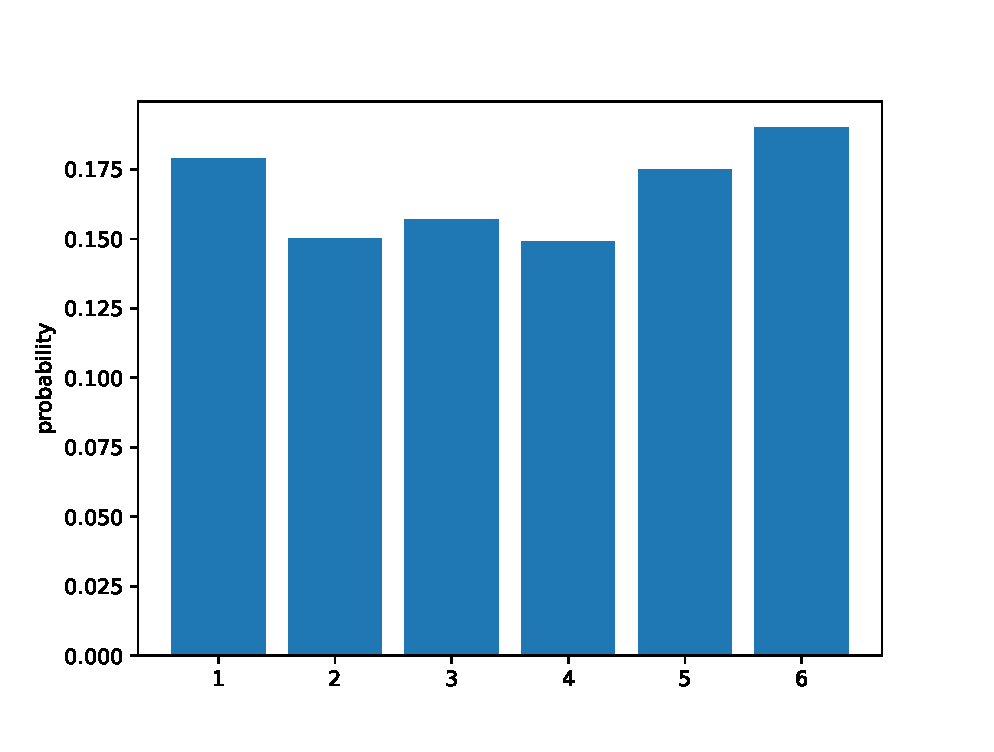
\includegraphics[width=\columnwidth]{./figures/probexm/probexm3.eps}
	\caption{probability of outcome of biased dice }
	\label{fig:bts3}
	\begin{lstlisting}
	figs/probexm/probexm3.eps
	\end{lstlisting}
\end{figure}
\begin{align}
P\left(D\right) &= \frac{149}{1000}
\\
&= 0.149
\end{align}
\item
NO of experiment with output 5 on dice = 175
\\
probability of outcome 5 = P(X=5)
\begin{align}
P\left(X=5\right) &= \frac{175}{1000}
\\
&= 0.175
\end{align}
\item
NO of experiment with output 6 on dice = 190
\\
probability of outcome 6 = P(X=6)
\begin{align}
P\left(X=6\right) &= \frac{190}{1000}
\\
&= 0.19
\end{align}
\end{enumerate}